\chapter{Objetivos}
\label{ch:Objetivos}

En este proyecto se construirán escenarios para la enseñanza utilizando diversas tecnologías. Para poder saber cual es el marco de desarrollo y donde se engloban los conceptos utilizados vamos a introducir algunos términos que servirán como contexto y que nos permitirán entender mejor de dónde surge la necesidad de estos escenarios y cual es la utilidad de los mismos.

\section{Descripción del problema}
\label{sec:obj_descripcionproblema}

El objetivo principal de este trabajo consiste en ampliar la colección de prácticas de JdeRobot-Academy, enriqueciéndolas y aumentando el abanico de posibilidades que se ofrece al alumno. Para ello necesitamos entender el funcionamiento tanto de JdeRobot como de ROS y familiarizarnos con el manejo de programas de edición 3D. Este objetivo lo hemos dividido en tres principales:
\begin{itemize}
	\item Creación de mundo más realista para Gazebo: Crearemos un modelo 3D de un escenario real para realizar las prácticas, en este caso del circuito de Fórmula 1 de Mónaco. Elegimos éste por ser un circuito conocido, corto tanto en su longitud como en el área que ocupa, y por estar ubicado en un entorno urbano y montañoso, lo que hace que sea estrecho y con subidas y bajadas. Lo prepararemos para algún tipo específico de práctica, añadiendo barreras en los bordes de la pista o marcas en el asfalto, y lo construiremos de forma que sea sencillo realizar futuras modificaciones para otros tipos de prácticas.
	
	\item Buscar un brazo robótico: Buscaremos un brazo robótico que funcione en Gazebo y bajo ROS o, si es posible, JdeRobot, y que cumpla con los requisitos impuestos. Estudiaremos además su construcción y su funcionamiento, y su comportamiento tanto de bajo como de alto nivel.
	
	\item Crear un controlador para el brazo robótico: Una vez encontrado un brazo adecuado y estudiado su funcionamiento, construiremos un controlador de bajo nivel que actúe directamente sobre las partes móviles del brazo, es decir, que mueva las articulaciones una a una. Crearemos una ventana con unos controles intuitivos para facilitar el manejo del robot.
\end{itemize}

\section{Requisitos}
\label{sec:obj_requisitos}
 Para alcanzar los objetivos marcados, nuestro proyecto deberá cumplir unos requisitos:
\begin{itemize}
	\item El desarrollo de este proyecto se hará bajo la arquitectura de JdeRobot en su última versión, la 5.5, así como de Gazebo 7 y de ROS Kinetic. Los componentes software se programarán utilizando principalmente Python, y en aquellos casos que no sea posible, utilizando el lenguaje principal de la plataforma o del tipo de archivo necesario.
	
	\item Los mundos creados se harán replicando el esquema de los ya existentes y se incorporarán al repositorio oficial de JdeRobot, por lo que debe ser posible utilizarlos junto con la plataforma de forma eficiente.
	
	\item El controlador debe ser de bajo nivel, esto es, no se apoyará en software de terceros ni plugins ni \textit{middleware}, debe funcionar directamente sobre el robot.
\end{itemize}



\section{Metodología}
\label{sec:obj_metodologia}


En el desarrollo del software de los componentes de nuestro trabajo utilizamos un  modelo de ciclo de vida en espiral. Es un modelo de proceso de software evolutivo, desarrollado por primera vez por Barry Boehm en 1988. En este modelo las actividades a realizar se conforman siguiendo una espiral, en la que cada bucle o iteración representa un conjunto de actividades que completan un modelo del proyecto final. Proporciona un modo de desarrollo evolutivo con un coste y complejidad incremental. 

Usando este modelo, al final de cada iteración obtenemos un prototipo funcional que cumple los requisitos marcados para esa iteración, lo que nos permite desarrollar poco a poco los objetivos. De esta manera aseguramos funcionalidades en cada paso y llevamos un seguimiento más preciso de fallos y bugs. También nos permite adaptarnos mejor a cambios de planificación y de requisitos.

\begin{figure}[hb]
	\centering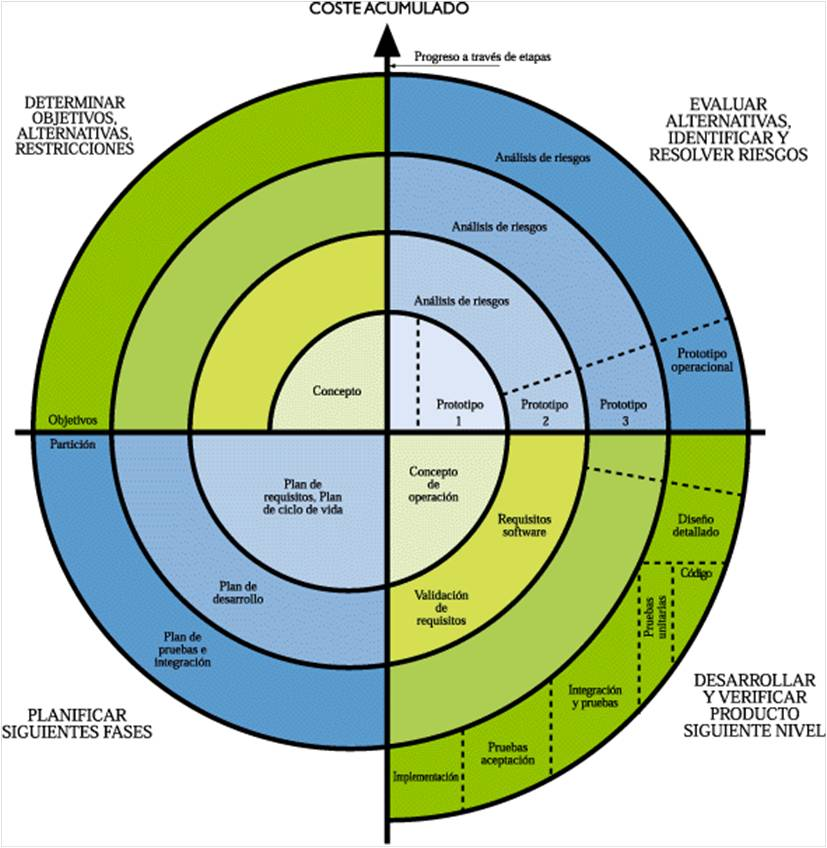
\includegraphics[width=0.7\textwidth]{espiral.jpg}
	\caption{Modelo de civlo de vida en espiral.}
	\label{fig:espiral}
\end{figure}

En cada vuelta de la espiral se parte de los resultados obtenidos en la anterior y se aumenta la complejidad. Dentro de cada vuelta se siguen una serie de pasos o tarear que guían el desarrollo del proyecto en cada iteración, como muestra el esquema que podemos ver en la figura \ref{fig:espiral}, Los pasos son:
\begin{enumerate}[1.]
	\item Determinar objetivos, alternativas, restricciones: En este paso se definen los objetivos específicos que tendremos que cumplir en cada iteración teniendo en mente el resultado final del proceso. Además se diseña una planificación detallada de gestión y se identifican las posibles alternativas. 
	
	\item Evaluar alternativas, identificar y resolver riesgos: Se efectúa un análisis detallado de las posibles alternativas que nos permitan cumplir los objetivos marcados utilizando distintos puntos de vista. Además se tienen en cuenta los riesgos del proceso, se elige la mejor estrategia teniendo en cuenta las dificultades que puedan surgir y se plantean estrategias alternativas para paliar el impacto de estos problemas.
	
	\item Desarrollar y verificar producto: Se desarrolla el producto de acuerdo a la planificación efectuada apuntando a los objetivos propuestos dentro del ciclo. Seguidamente probamos que el resultado sea satisfactorio de acuerdo a dichos objetivos.
	
	\item Planear las siguientes fases: Se revisa el proyecto y se decide si continuar con un nuevo ciclo de la espiral. En caso afirmativo se desarrollan los planes para la siguiente iteración y se subsanan los posibles errores cometidos en la última iteración.
	
\end{enumerate}

Las fases de desarrollo seguidas en el proyecto se corresponden con los pasos seguidos en los siguientes capítulos. Se han realizado reuniones semanales con el tutor para mantener un seguimiento y una progresión adecuada en el desarrollo del proyecto, alcanzando los objetivos marcados y estudiando diferentes alternativas para conseguirlos.

Para tener constancia de los progresos y del desarrollo general del proyecto se ha utilizado un apartado en la propia página de JdeRobot, un MediaWiki\cite{mediawiki} donde ir documentando periódicamente los progresos, incluyendo fotos y vídeos de los logros conseguidos y de los problemas encontrados. Ha servido como referencia para que las reuniones con el tutor estén sincronizadas, y a modo de diario para mantener un registro de los progresos y de las dificultades encontradas. También se ha utilizado un repositorio en GitHub\cite{mirepo} donde se encuentran todos los archivos relacionados con el proyecto, desde test y tutoriales hasta el código fuente del resultado final, pasando por alternativas descartadas y pruebas fallidas.





























